\documentclass{article}
\usepackage[T1]{fontenc}
\usepackage[ansinew ]{inputenc}
\usepackage{amsmath}
\usepackage{tikz}
\usepackage{tikzsymbols}
\usepackage{lmodern}
\usetikzlibrary{arrows,automata}
\setlength\parindent{0pt}

\begin{document}

\begin{center}
  \Large{Informatik D - �bungsblatt 3}

  \large{Sebastian H�ffner, Andrea Suckro}
\end{center}


\section{Aufgabe 3.1}
Sei $L \subseteq \Sigma^{*}$ eine endliche Sprache, d.h. eine Sprache mit endlicher Anzahl W�rtern $\omega \in L$ endlicher L�nge. Dann k�nnen wir eine Grammatik definieren, die individuell alle W�rter aus $L$ generiert.
\begin{align*}
S\ \rightarrow\ \omega_i\ |\ \omega_{i+1}\ |\ ...
\end{align*}
Diese Grammatik kann in eine regul�re Grammatik �berf�hrt werden, indem jedes Wort $\omega_i$ als Verkettung von Regeln dargestellt wird.
\begin{align*}
S\ &\rightarrow\ O_{i,0}\ |\ O_{i+1,0}\ |\ ...\\
O_{i,0}\ &\rightarrow\ \omega_{i,0} O_{i,1} \\
O_{i,1}\ &\rightarrow\ \omega_{i,1} O_{i,2} \\
...
\end{align*}
In der Vorlesung wurde bereits gezeigt, dass regul�re Grammatiken in regul�re Ausdr�cke und endliche Automaten �berf�hrt werden k�nnen, also ist die endliche Sprache ebenfalls regul�r.


\section{Aufgabe 3.2}
\subsection{Aufgabe 3.2 (a)}
\begin{align*}
Z_1 &\rightarrow\ 1\ |\ 1Z_2 \\
Z_2 &\rightarrow\ 1\ |\ 1Z_2\ |\ 0Z_3 \\
Z_3 &\rightarrow\ 1\ |\ 0Z_1
%Z_4 &\rightarrow\ 
\end{align*}

\subsection{Aufgabe 3.2 (b)}
\begin{center}
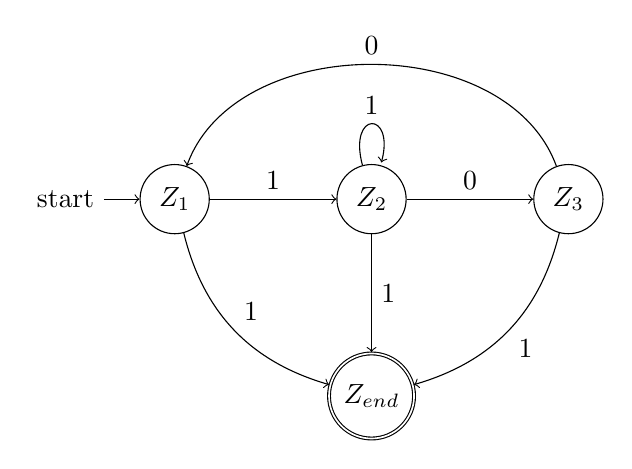
\begin{tikzpicture}[->, auto, node distance=2.5cm]
  \node[initial,state]   (Z1)               {$Z_1$};
  \node[state]           (Z2) [right of=Z1] {$Z_2$};
  \node[state]           (Z3) [right of=Z2] {$Z_3$};
  \node[state,accepting] (Ze) [below of=Z2] {$Z_{end}$};

  \path (Z1) edge [bend right]           node {1} (Ze)
             edge                        node {1} (Z2)
        (Z2) edge                        node {1} (Ze)
             edge [loop above]           node {1} (Z2)
             edge                        node {0} (Z3)
        (Z3) edge [bend left]            node {1} (Ze)
             edge [above, bend right=70] node {0} (Z1)
        ;
\end{tikzpicture}
\end{center}


\section{Aufgabe 3.3}
\begin{center}
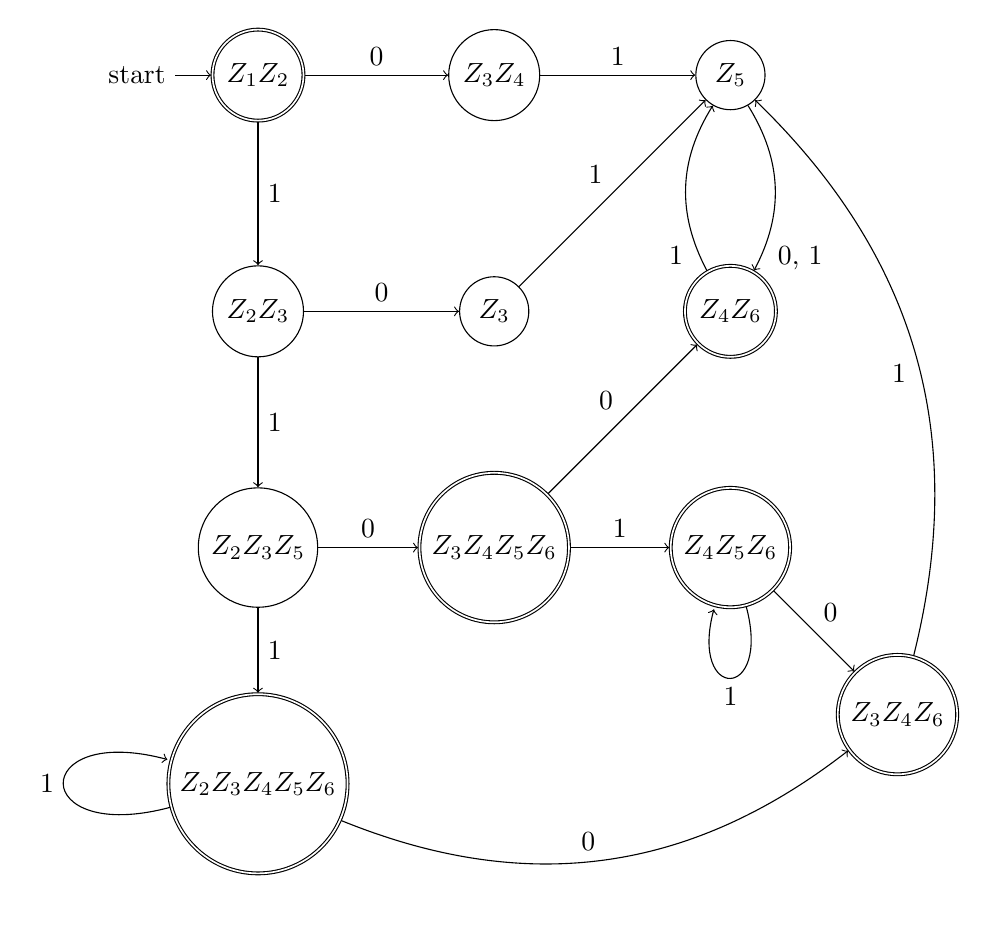
\begin{tikzpicture}[->, auto, node distance=3cm]
  \node[initial,state,accepting] (Z1Z2)                               {$Z_1Z_2$};
  \node[state]                   (Z2Z3)       [below of=Z1Z2]         {$Z_2Z_3$};
  \node[state]                   (Z2Z3Z5)     [below of=Z2Z3]         {$Z_2Z_3Z_5$};
  \node[state,accepting]         (Z2Z3Z4Z5Z6) [below of=Z2Z3Z5]       {$Z_2Z_3Z_4Z_5Z_6$};
  \node[state]                   (Z3)         [right of=Z2Z3]         {$Z_3$};
  \node[state]                   (Z3Z4)       [right of=Z1Z2]         {$Z_3Z_4$};
  \node[state,accepting]         (Z3Z4Z5Z6)   [right of=Z2Z3Z5]       {$Z_3Z_4Z_5Z_6$};
  \node[state,accepting]         (Z4Z5Z6)     [right of=Z3Z4Z5Z6]     {$Z_4Z_5Z_6$};
  \node[state,accepting]         (Z4Z6)       [right of=Z3]           {$Z_4Z_6$};
  \node[state]                   (Z5)         [right of=Z3Z4]         {$Z_5$};
  \node[state,accepting]         (Z3Z4Z6)     [below right of=Z4Z5Z6] {$Z_3Z_4Z_6$};

  \path (Z1Z2)       edge [] node {0} (Z3Z4)
                     edge [] node {1} (Z2Z3)
        (Z2Z3)       edge [] node {0} (Z3)
                     edge [] node {1} (Z2Z3Z5)
        (Z2Z3Z5)     edge [] node {0} (Z3Z4Z5Z6)
                     edge [] node {1} (Z2Z3Z4Z5Z6)
        (Z2Z3Z4Z5Z6) edge [bend right] node {0} (Z3Z4Z6)
                     edge [loop left]  node {1} (Z2Z3Z4Z5Z6)
        (Z3)         %edge [] node {0} ()
                     edge [] node {1} (Z5)
        (Z3Z4)       %edge [] node {0} ()
                     edge [] node {1} (Z5)
        (Z3Z4Z5Z6)   edge [] node {0} (Z4Z6)
                     edge [] node {1} (Z4Z5Z6)
        (Z4Z5Z6)     edge []           node {0} (Z3Z4Z6)
                     edge [loop below] node {1} (Z4Z5Z6)
        (Z4Z6)       %edge [] node {0} ()
                     edge [bend left, pos=0.2] node {1} (Z5)
        (Z5)         %edge [] node {0} (Z4Z6)
                     %edge [] node {1} (Z4Z6)
                     edge [bend left, pos=0.8] node {0, 1} (Z4Z6)
        (Z3Z4Z6)     %edge [] node {0} ()
                     edge [bend right] node {1} (Z5)
        ;
\end{tikzpicture}
\end{center}


\section{Aufgabe 3.4}


\section{Aufgabe 3.5}
%\begin{figure}[h]
%  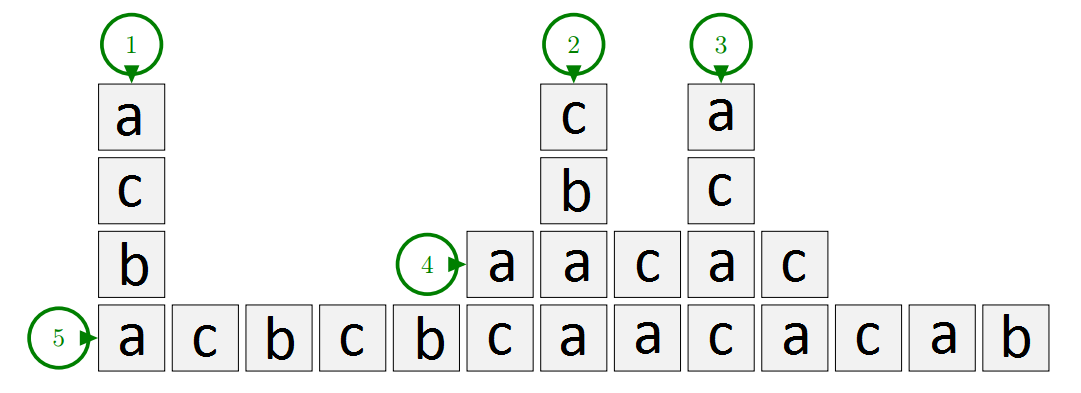
\includegraphics[width=\textwidth]{crossword.png}
%\end{figure}
\begin{enumerate}
	\item bbbbb
  \item bcbca
  \item bdda
  \item adadc
  \item bbaadd
\end{enumerate}


\section{Aufgabe 3.6}


\end{document}